% --------------------------------------------------------------
% This is all preamble stuff that you don't have to worry about.
% Head down to where it says "Start here"
% --------------------------------------------------------------

\documentclass[12pt]{article}

\usepackage[margin=1in]{geometry}
\usepackage{amsmath,amsthm,amssymb}
\usepackage{tikz}

\newcommand{\N}{\mathbb{N}}
\newcommand{\Z}{\mathbb{Z}}

\newenvironment{theorem}[2][Theorem]{\begin{trivlist}
\item[\hskip \labelsep {\bfseries #1}\hskip \labelsep {\bfseries #2.}]}{\end{trivlist}}
\newenvironment{lemma}[2][Lemma]{\begin{trivlist}
\item[\hskip \labelsep {\bfseries #1}\hskip \labelsep {\bfseries #2.}]}{\end{trivlist}}
\newenvironment{exercise}[2][Exercise]{\begin{trivlist}
\item[\hskip \labelsep {\bfseries #1}\hskip \labelsep {\bfseries #2.}]}{\end{trivlist}}
\newenvironment{question}[2][Question]{\begin{trivlist}
\item[\hskip \labelsep {\bfseries #1}\hskip \labelsep {\bfseries #2.}]}{\end{trivlist}}
\newenvironment{proposition}[2][Proposition]{\begin{trivlist}
\item[\hskip \labelsep {\bfseries #1}\hskip \labelsep {\bfseries #2.}]}{\end{trivlist}}
\newenvironment{corollary}[2][Corollary]{\begin{trivlist}
\item[\hskip \labelsep {\bfseries #1}\hskip \labelsep {\bfseries #2.}]}{\end{trivlist}}

\begin{document}

% --------------------------------------------------------------
%                         Start here
% --------------------------------------------------------------

%\renewcommand{\qedsymbol}{\filledbox}

\title{Homework 3}%replace X with the appropriate number
\author{Dustin Lambright - dalambri \\ Aseem Raina - araina \\ Bihan Zhang - bzhang28\\ %replace with your name
CSC 565 - Graph Theory} %if necessary, replace with your course title

\maketitle


\begin{question}{1}
Show that every simple graph $G$ with 6 vertices has either a clique of size 3 or an independent
set of size 3.
\end{question}

By the definition of inependent sets and cliques, any graph G with a clique of size n will also have a clique of n-1, n-2, ... n-(n-1).  The same goes for an independent set.  Therefore, using contradiction, if a graph does not have a clique of size 3 and does not have an independent set of size 3, the statement is false. \\ \\

The graph $K_{1,5}$ has a maximum clique size of 2, but an independent set of 5. (displayed in red)
\begin{align*}
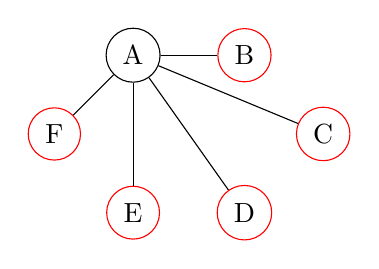
\begin{tikzpicture}
\node[shape=circle,draw=black] (A) at (1,2) {A};
\node[shape=circle,draw=red] (B) at (2.4142857,2) {B};
\node[shape=circle,draw=red] (C) at (3.4142856,1) {C};
\node[shape=circle,draw=red] (D) at (2.4142857,0) {D};
\node[shape=circle,draw=red] (E) at (1,0) {E};
\node[shape=circle,draw=red] (F) at (0,1) {F};
\path [] (A) edge node[left] {} (B);
\path [] (A) edge node[left] {} (C);
\path [] (A) edge node[left] {} (D);
\path [] (A) edge node[left] {} (E);
\path [] (A) edge node[left] {} (F);
\end{tikzpicture}
\end{align*}

In an effort to reduce the size of the maximum independent set, edges are replaced, creating a cyclic graph: \\

\begin{align*}
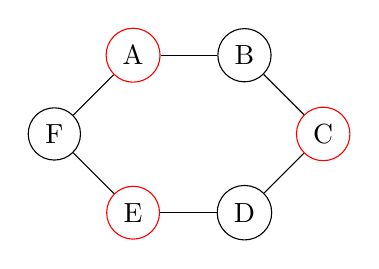
\begin{tikzpicture}
\node[shape=circle,draw=red] (A) at (1,2) {A};
\node[shape=circle,draw=black] (B) at (2.4142857,2) {B};
\node[shape=circle,draw=red] (C) at (3.4142856,1) {C};
\node[shape=circle,draw=black] (D) at (2.4142857,0) {D};
\node[shape=circle,draw=red] (E) at (1,0) {E};
\node[shape=circle,draw=black] (F) at (0,1) {F};
\path [] (A) edge node[left] {} (B);
\path [] (B) edge node[left] {} (C);
\path [] (C) edge node[left] {} (D);
\path [] (D) edge node[left] {} (E);
\path [] (F) edge node[left] {} (A);
\path [] (E) edge node[left] {} (F);
\end{tikzpicture}
\end{align*}

This graph has a a maximum independent set of 3, and a maximum clique of 2. The only way to reduce the size of an independent set, i.e., $\{A,E,C\}$ is to connect any of those vertices with an edge.  The connection of any of these vertices results in a clique of size 3.  In an effort to maintain our clique constraint, if we remove the edges AF and AB to connect the independent set $\{A,E,C\}$, we end up with an independent set $\{A,F,B, D\}$.

\begin{align*}
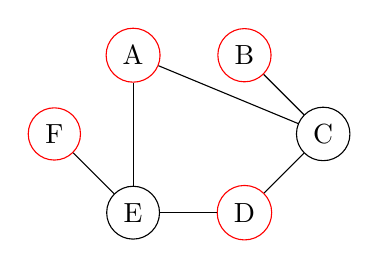
\begin{tikzpicture}
\node[shape=circle,draw=red] (A) at (1,2) {A};
\node[shape=circle,draw=red] (B) at (2.4142857,2) {B};
\node[shape=circle,draw=black] (C) at (3.4142856,1) {C};
\node[shape=circle,draw=red] (D) at (2.4142857,0) {D};
\node[shape=circle,draw=black] (E) at (1,0) {E};
\node[shape=circle,draw=red] (F) at (0,1) {F};
\path [] (A) edge node[left] {} (C);
\path [] (B) edge node[left] {} (C);
\path [] (C) edge node[left] {} (D);
\path [] (D) edge node[left] {} (E);
\path [] (E) edge node[left] {} (A);
\path [] (E) edge node[left] {} (F);
\end{tikzpicture}
\end{align*}

The graph $C_6$ is the closest we can get to a graph without a clique of size 3 and without an independent set of size 3, but it has an independent set of size three, proving that a graph with a vertex count of 6 has to have an independent set of size 3 or a clique of size 3.

% --------------------------------------------------------------
%     You don't have to mess with anything below this line.
% --------------------------------------------------------------

\end{document}
